% Straight up stealing preamble from Eli Holmes 
%%%%%%%%%%%%%%%%%%%%%%%%%%%%%%%%%%%%%%START PREAMBLE THAT IS THE SAME FOR ALL EXAMPLES
\documentclass{article}

%Required: You must have these
\usepackage{Sweave}
\usepackage{graphicx}
\usepackage{tabularx}
\usepackage{hyperref}
\usepackage{natbib}
\usepackage{pdflscape}
\usepackage{array}
\usepackage{gensymb}
%\usepackage[backend=bibtex]{biblatex}
%Strongly recommended
  %put your figures in one place
%\SweaveOpts{prefix.string=figures/, eps=FALSE} 
%you'll want these for pretty captioning
\usepackage[small]{caption}

\setkeys{Gin}{width=0.8\textwidth}  %make the figs 50 perc textwidth
\setlength{\captionmargin}{30pt}
\setlength{\abovecaptionskip}{10pt}
\setlength{\belowcaptionskip}{10pt}
% manual for caption  http://www.dd.chalmers.se/latex/Docs/PDF/caption.pdf

%Optional: I like to muck with my margins and spacing in ways that LaTeX frowns on
%Here's how to do that
 \topmargin -1.5cm        
 \oddsidemargin -0.04cm   
 \evensidemargin -0.04cm  % same as oddsidemargin but for left-hand pages
 \textwidth 16.59cm
 \textheight 21.94cm 
 %\pagestyle{empty}       % Uncomment if don't want page numbers
 \parskip 7.2pt           % sets spacing between paragraphs
 %\renewcommand{\baselinestretch}{1.5} 	% Uncomment for 1.5 spacing between lines
\parindent 0pt% sets leading space for paragraphs
\usepackage{setspace}
%\doublespacing

%%%%%%%%%%%%%%%%%%%%%%%%%%%%%%%%%%%%%%END PREAMBLE THAT IS THE SAME FOR ALL EXAMPLES

%Start of the document
\begin{document}

\bibliographystyle{/Users/aileneettinger/citations/Bibtex/styles/amnat.bst}
\title{Supplemental Materials for: How do climate change experiments alter plot-scale climate?} 

\author{A.K. Ettinger, I. Chuine, B. Cook, J. Dukes, A.M. Ellison, M.R. Johnston, A.M. Panetta,\\ C. Rollinson, Y. Vitasse, E. Wolkovich}
%\date{\today}
\maketitle  %put the fancy title on
%\tableofcontents      %add a table of contents
%\clearpage
%%%%%%%%%%%%%%%%%%%%%%%%%%%%%%%%%%%%%%%%%%%%%%%%%%%
\renewcommand{\thetable}{S\arabic{table}}
\renewcommand{\thefigure}{S\arabic{figure}}

\section* {Additional methods for database development}
For our literature review, we searched Web of Science (ISI) for Topic=(warm* OR temperature*) AND Topic=(plant* AND phenolog*) AND Topic=(experiment* OR manip*). We restricted dates to the time period after the STONE database (i.e., January 2011 through March 2015). This yielded 277 new studies. We removed all passive warming studies from the list, and contacted authors for daily data. Three additional datasets were offered or suggested to us, and in March 2018, we added additional studies found by using the same terms to search the following online databases for additional datasets: dataONE (https://search.dataone.org/), KNB (https://knb.ecoinformatics.org/), and dryad (https://www.datadryad.org/). The resulting database contains daily climate data collected between 1991 and 2015 from 15 North American, European, and Chinese climate change experiments (Table \ref{tab:methods}, Figure \ref{fig:map}). %We were unable to include the following studies because authors declined to share their data or did not respond: \citep{schwartzberg2014,moser2011,caron2015,ellebjerg2008}.

\section* {Details of statistical analyses and results}
For all analyses, we use mixed-effects models implemented with the lme4 package in R, version 3.2.4 \citep{bates2015,rcoreteam2017}. Mixed-effects models, also called multi-level or hierarchical models, can account for structured data that violate the independence assumption of traditional linear regression \citep{gelman2007}. In our analyses, we use levels/groupings of experimental site, year, and day of year (doy) to account for this mutual dependence among data points. We use three as a minimum threshold for sample size within each level/grouping, for fixed and random effects (i.e., there must be atleast three observations within each level/group for it to be considered as a separate group in our analyses). To test for significance of fixed effects in our models, we use Type II tests for models including only main effects and Type III tests for models including interactions, as well as main effects. 
\subsection* {Analysis of effects of warming on daily temperature range}
To test how active warming alters daily temperature range (DTR, the difference between maximum and minimum temperatures in a day), we used data from eight studies in the MC3E database that include daily measurements of soil and/or above-ground (i.e., air, canopy, surface) temperature maxima and minima. These studies included infrared (n=4), forced air (n=2), and combined forced air and soil cable (n=2) warming types.  For consistency, we included only structural controls (we therefore excluded exp15, which used only ambient controls), and also excluded data from plots with precipitation treatments. We fit linear mixed-effect models with above-ground DTR, soil DTR, minimum and maximum daily above-ground temperature, and minimum and maximum daily soil temperature as response variables. We included target temperature treatment (or measured temperature, for those studies that did not have explicit target temperatures) as a predictor (i.e., a fixed effect). Random effects were site and study year nested within site (with random slopes and intercepts, Tables \ref{table:dtrtemp} \& \ref{table:sdtrtemp}). 

\subsection* {Analysis of effects of time and space on experimental microclimate}
To test how treatment effects vary spatially (i.e., among blocks within a study) and temporally (i.e., among years within a study), we used data from the four studies in the MC3E database that used blocked designs. These studies included infrared (n=5), and soil cable (n=1) warming types.  We fit linear mixed-effect models with mean daily soil temperature, minimum daily air temperature, and maximum daily air temperature as response variables (Figure 3 in the main text). For temporal models, we included fixed effects of temperature treatment, year, and their interaction; random effects were site and block nested within site (intercept-only structure, Table \ref{table:blocks_time}). For spatial models, we included fixed effects of temperature treatment, block, and their interaction; random effects were site and year nested within site (intercept-only structure, Table \ref{table:blocks_space}). Both of these models excluded data from plots with precipitation treatments. 
\subsection* {Analysis of effects of infrastructure on experimental microclimate}
To test how infrastructure affects microclimate, we compared temperature and soil moisture data from the studies in the MC3E database that monitored climate in two types of control plots: structural controls (i.e., `shams' or `disturbance controls,'which contained all the warming infrastructure, such as soil cables or forced air chambers with no heat applied) and ambient controls with no infrastructure added. These five studies consisted of soil cables (n=1), forced air (n=2), and combined soil and forced air (n=2) warming types and occurred at two sites: Duke Forest and Harvard Forest \citep{farnsworth1995,clark2014a,marchin2015,pelini2011}. One additional study, exp15, which utilized forced air, monitored environmental conditions in both ambient and structural controls, but we were only able to obtain data for the ambient controls so it is excluded from this analysis. Note that all studies that employ forced air warming utilize chambers, whereas the other warming types did not utilize chambers.
\par We fit linear mixed-effects models by month for the following response variables: mean daily soil temperature, minimum and maximum daily air and soil temperature (\citet{farnsworth1995} only measured mean soil, so there are only four different studies in models for minimum and maximum air and soil), and soil moisture. The predictor was control type (sham or ambient). To allow for both mean differences in temperature and the effect of control to to vary among sites and years, random effects were site and year nested within site, modeled as random slopes and random intercepts. 
We found that experimental structures altered above-ground and soil temperatures in opposing ways: above-ground temperatures were higher in the structural controls, compared with ambient conditions with no structures installed, whereas soil temperatures were lower in the structural controls compared with ambient soil (Figure 3 in the main text).  In addition, soil moisture was lower in structural controls compared with ambient conditions. These general patterns were consistent across the different temperature models we fit (mean, minimum, and maximum soil and air temperatures), although the magnitude varied across months, as well as among studies. We show summaries from models fit to the entire year (Tables \ref{table:shamamb_soiltemp}, \ref{table:shamamb_airtemp}, \ref{table:shamamb_soilmois}), as well as summaries from models fit to each month of data, as is shown in Figure 3 in the main text (Tables \ref{table:shamamb_stempm}, \ref{table:shamamb_atempm}, \ref{table:shamamb_soilmoism}).

\par For experiments using infrared heating, we were unable to directly compare ambient and structural controls because no studies in our database included and shared data from both control types. Instead, we compared differences between each control type (ambient versus structural) and the measured amount of warming per degree of target warming in experimental plots. We predicted that, if heating infrastructure affects microclimate, the measured amount of warming per degree of target warming should differ by control type. Of the seven infrared sites in our database that measured soil temperature, three used ambient controls (exp06, exp11, exp14) and four used structural controls (exp01, exp09, exp12, exp13).  Among these studies, warming per \degree of target warming was 1.01 for structural controls (SE= 0.09, Table  \ref{table:infrared}), but significantly lower for ambient controls (0.41 \degree C of warming per \degree C of target warming, SE=0.09, Table \ref{table:infrared}). This trend, based on a limited number of studies and sites, suggests that infrared heating equipment may alter microclimate, likely by shading the soil surface \citep{mcdaniel2014}.  

\subsection* {Analysis of effects of precipitation treatments on above-ground temperature}
Of the 15 experiments in the MC3E database, four manipulated precipitation and measured above-ground temperature and three of these also measured soil temperature (all four studies used infrared warming). To examine the effects of precipitation treatment on temperature, we fit linear mixed-effects models to data from these sites with temperature (above-ground daily minimum and maximum, and soil minimum and maximum) as the response variables. Predictors were precipitation treatment (a continuous fixed effect, which ranged from 50 to 200\% of ambient for these four studies), target warming (a continuous fixed effect, which ranged from 0 to 4 \degree C for these four studies), and their interaction. To account for methodological and other differences among sites, we included site as a random effect, with year and doy nested within site to account for the non-independent nature of measurements taken on the same day within sites. We used a random intercept model structure (Table \ref{table:preciptemp}). 

\subsection* {Analysis of effects of experimental warming on soil moisture}
Of the 15 experiments in the MC3E database, 12 measured and reported soil moisture. These studies included infrared (n=7), forced air (n=3), and combined forced air and soil cable (n=2) warming types. To examine the effects of target warming treatment on soil moisture, we fit linear mixed-effects models to data from these ten sites, excluding plots with precipitation treatments. We first fit a model with soil moisture as the response and a predictor of target warming (a continuous fixed effect, which ranged from 0 to 5.5 \degree C for these 12 studies). To account for differences among warming types, we included warming type as a fixed effect, grouping combined forced air/soil cable warming type with forced air studies because of the low sample size in this group. We accounted for other differences among studies by including site as a random effect, with year and doy nested within site to account for the non-independent nature of measurements taken on the same day within sites.  We used a random intercept model structure (Table \ref{table:targsoilmois}). 

\par In addition to testing how experimental warming influenced soil moisture, we also tested how experimental structures influenced soil moisture. We compared the soil moisture measured in structural controls to both ambient controls and warmed plots by fitting a model with categorical fixed effects of ``ambient," ``structural control," and ``warmed."  We again included warming type as a fixed effect, and site as a random effect, with doy nested within site to account for the non-independent nature of measurements taken on the same day within sites, and used a random intercept structure (Table \ref{table:warmsoilmois}). 

\subsection* {Analysis of budburst phenology}
We wanted to investigate how using measured plot-level climate variables, as opposed to target warming, alters estimates of temperature sensitivity in ecology. To do this, we fit two different types of models to data from the five study sites in the MC3E database that recorded above-ground temperature and soil moisture, as well as phenology data (doy of budburst). These studies included infrared (n=1), forced air (n=2), and combined forced air and soil cable (n=2) warming types. We used only structural controls in the reported analysis, because this is the type of control that all five studies posess(including ambient control plots in the analysis did not qualitatively change the results). We focus on budburst, as this phenological phase was reported most commonly among studies in the MC3E database. For all models, we accounted for non-independence by including species, site, and year nested within site as intercept-only random effects (Table \ref{table:bbmods}). The target warming model included only one explanatory variable (the target amount of warming).  We compared this to models with mean annual measured above-ground temperature (offset by subtracting the minimum temperature across all studies and plots, to make model intercepts more similar), mean winter (January-March) soil moisture, and their interaction as explanatory variables. The slope for temperature in the measured climate model can be directly compared to the slope for target warming in the target warming model because the units are the same (change in budburst, in days, per\degree C).
\par To determine which specific above-ground temperature variable to include in the measured climate model, we compared AICs of models for with four different temperature variables (mean annual minimum and maximum temperatures, mean January-March minimum and maximum temperatures). The model with mean annual minimum temperature, mean January-March soil moisture, and their interaction provided the best model fit (lowest AIC, highest explained variation, Table \ref{table:bbaic}), so we discuss and interpret that model in the main text, summarize it in Table \ref{table:bbmods}, and present its coefficients in Figure 6. 

\bibliography{/Users/aileneettinger/citations/Bibtex/mylibrary}
\clearpage
\section* {Supplemental Tables} 
\begin{landscape}
\begin{footnotesize} 
% latex table generated in R 3.4.2 by xtable 1.8-2 package
% Tue Jul 10 13:08:29 2018
\begin{table}[ht]
\centering
\caption{\textbf{Experimental sites included in the MC3E database}. Experimental sites correspond to the map (Figure 1, main text). We give the study ID, location, source, years of data included, warming type, the type of control used to maintain warming, plot area (in square meters), watts of heating output, target warming treatment (\degree C; reported warming was used for exp06, exp11, exp12, and for the two lower warming treatments for exp01, all of which did not have explicit targets for any treatments), precipitation treatment (proportion of ambient), method of above-ground temperature measurement (with height of measurement, in cm, for air), depth of soil temperature measurement (cm), depth of soil moisture measurement (cm) used in each study, the type(s) of control plots installed (structural controls contain all the warming infrastructure, such as soil cables, but with no heat applied; ambient controls have no infrastructure added), and statistical analysis used in the source listed (i.e., ANOVA with categorical explatory variables for different warming levels versus continuous microclimate explanatory variables). All studies that employ forced air warming utilize chambers, whereas the other warming types did not utilize chambers. Note that some sites may have multiple sources; however, we list only one here.} 
\label{tab:methods}
\begingroup\footnotesize
\begin{tabular}{|p{0.04\textwidth}|p{0.15\textwidth}|p{0.12\textwidth}|p{0.04\textwidth}|p{0.07\textwidth}|p{0.07\textwidth}|p{0.03\textwidth}|p{0.03\textwidth}|p{0.07\textwidth}|p{0.07\textwidth}|p{0.07\textwidth}|p{0.04\textwidth}|p{0.04\textwidth}|p{0.08\textwidth}|p{0.08\textwidth}|}
  \hline
study & location & source & data years & warming type & warming control & area & watts & warming trtmt & precip trtmt & above-ground temp & soil temp depth & soil moist depth & control type & analysis type \\ 
  \hline
exp01 & Waltham, MA, USA & Hoeppner and Dukes 2012 & 2009-2011 & infrared & feedback & 4.00 & 50, 150, 250 & 1, 2.7, 4 & 0.5, 1.0, 1.5 & canopy & 2, 10 & 30 & structural & categorical \\ 
   \hline
exp02 & Montpelier, France & Morin et al. 2010 & 2004 & infrared & feedback & 1.56 & 102.4 & 1.5, 3 & 0.7, 1.0 &   &   & 15, 30 & ambient & categorical \\ 
   \hline
exp03 & Duke Forest, NC, USA & Clark et al. 2014 & 2009-2014 & forced air and soil & feedback & 17.00 &  & 3, 5 &   & air (30) & 10 & 30 & both & continuous \\ 
   \hline
exp04 & Harvard Forest, MA, USA & Clark et al. 2014 & 2009-2012 & forced air and soil & feedback & 17.00 &  & 3, 5 &   & air (30) & 10 & 30 & both & continuous \\ 
   \hline
exp05 & Jasper Ridge Biological Preserve, CA, USA & Cleland et al. 2007 & 1998-2002 & infrared & constant & 3.14 & 80 & 1.5 & 1.0, 1.5 &   & 15 & 15 & ambient & categorical \\ 
   \hline
exp06 & Rocky Mountain Biological Lab, CO, USA & Dunne et al. 2003 & 1995-1998 & infrared &  & 30.00 & 22 & 1.9 &   &   & 12, 25 & 12, 25 & ambient & categorical \\ 
   \hline
exp07 & Harvard Forest, MA, USA & Pelini et al. 2011 & 2010-2015 & forced air & feedback & 15.70 &  & 1.5-5.5 &   & air (22) & 2, 6 & 30 & both & continuous \\ 
   \hline
exp08 & Harvard Forest, MA, USA & Farnsworth et al. 1995 & 1993 & soil warming &  & 36.00 &  & 5 &   &   & 5 &   & both & categorical \\ 
   \hline
exp09 & Stone Valley Forest, PA, USA & Rollinson and Kaye 2012 & 2009-2010 & infrared & feedback & 4.00 & 100 & 2 & 1.0, 1.2 & surface & 3 & 8 & structural & categorical \\ 
   \hline
exp10 & Duke Forest, NC, USA & Marchin et al. 2015 & 2010-2013 & forced air & feedback & 15.70 &  & 1.5-5.5 &   & air (22) & 2, 6 & 30 & both & continuous \\ 
   \hline
exp11 & Rocky Mountain Biological Lab, CO, USA & Price and Wasser 1998 & 1991-1994 & infrared & constant & 30.00 & 15 & 1.2 &   &   & 12 &   & ambient & categorical \\ 
   \hline
exp12 & Kessler Farm Field Laboratory, OK, USA & Sherry et al. 2007 & 2003 & infrared & constant & 6.00 & 100 & 4.17 & 1.0, 2.0 & air (14) & 7.5, 22.5 & 15 & structural & categorical \\ 
   \hline
exp13 & Haibei Alpine Grassland Research Station, China & Suonan et al. 2017 & 2012-2014 & infrared & constant & 3.96 & 303 & 1.5 &   & air (30) & 5, 10 & 5, 10 & structural & categorical \\ 
   \hline
exp14 & Cedar Creek, MN, USA & Whittington et al 2015 & 2009-2011 & infrared & constant & 7.50 & 80, 133 & 1.5, 3 &   & air (10,25) & 1, 10 & 6 & ambient & categorical \\ 
   \hline
exp15 & Oak Ridge, TN, USA & Gunderson et al 2015 & 2003-2005 & forced air & feedback & 9.42 &  & 2, 4 &   & air &   & 10, 20 & both & categorical \\ 
   \hline
\end{tabular}
\endgroup
\end{table}\end{footnotesize} 
\end{landscape}
\clearpage
\begin{footnotesize} 

% latex table generated in R 3.4.2 by xtable 1.8-2 package
% Tue Jul 10 13:08:52 2018
\begin{table}[ht]
\centering
\caption{\textbf{Summary of warming treatments, by warming type,} for studies included in the MC3E database. An additional common type of experimental warming, passive open-top chambers (OTC), is included for comparison. Summaries of the target warming treatments (\degree C) and measured warming for air temperature, soil surface temperature, and soil temperture are given. Measured warming shown here is for warming treatments only (precipitation treatments are expcluded), and is the difference between mean annual temperature (MAT) of control plots and MAT of each treatment level within a study. Mean difference (with standard error) and the range of differences (minimum to maximum differences in MAT) is shown. n is the number of studies of each warming type in the MC3E database. *Passive OTC data are from \cite{bokhorst2013}.} 
\label{tab:warmtreats}
\begingroup\footnotesize
\begin{tabular}{|p{0.20\textwidth}p{0.10\textwidth}p{0.10\textwidth}p{0.10\textwidth}p{0.10\textwidth}p{0.10\textwidth}|}
  \hline
temperature type & forced air & force air, soil cables & infrared & soil cables & passive otc \\ 
  \hline
target (min-max) & 3.5 (1.5-5.5) & 4 (3-5) & 2.2 (1-4) & 5 &   \\ 
  air, mean (se) & 3.22 (0.12) & 1.9 (0.24) & 1.08 (0.16) &  & 0.8 (0.1) \\ 
  air, range & 0.83-5.2 & -0.05-3.59 & 0.42-1.83 &  & 0.5-1.3 \\ 
  surface, mean (se) &  &  & 1.72 (0.1) &  & 0.9 (0.1) \\ 
  surface, range &  &  & 1.52-1.87 &  & 0.4-1.4 \\ 
  soil, mean (se) & 1.29 (0.09) & 3.01 (0.34) & 1.73 (0.2) & 5.04 & 0.8 (0.3) \\ 
  soil, range & -0.93-3.46 & 0.02-5.08 & -0.06-4.31 &   & -0.1-3.9 \\ 
  n & 2 & 2 & 9 & 1 & 0* \\ 
   \hline
\end{tabular}
\endgroup
\end{table}\end{footnotesize} 
\clearpage

% latex table generated in R 3.4.2 by xtable 1.8-2 package
% Tue Jul 10 13:08:52 2018
\begin{table}[ht]
\centering
\caption{\textbf{Summary of linear mixed-effects models of how target warming treatment affects above-ground daily temperature range (DTR), mimumim, and maximum temperatures in climate change experiments.} We excluded data from plots with precipitation treatments from these analyses. Estimates (est.) are the intercept and coefficient for target warming from the model; se is the standard error for these estimates. The effect of target warming on observed warming was significant based on Type II Wald $\chi^{2}$ tests of fixed effects for above-ground minimum temperature ($\chi^{2}$=46.58, df=1, p<0.001) and above-ground maximum temperature ($\chi^{2}$=5.74, df=1, p=0.02), but not for above-ground daily DTR ($\chi^{2}$=1.38, df=1, p=0.24).  Random effects were site (n=8), with a random slope and intercept structure (listed for each model), and year nested within site (n=32 year-site combinations, not shown). Total number of observations=169,797, and units are \degree C for all three models.} 
\label{table:dtrtemp}
\begingroup\footnotesize
\begin{tabular}{|p{0.19\textwidth}|p{0.07\textwidth}p{0.07\textwidth}|p{0.07\textwidth}p{0.07\textwidth}|p{0.07\textwidth}p{0.07\textwidth}|}
  \hline
  &\multicolumn{2}{c |}{above-ground DTR} &\multicolumn{2}{c |}{above-ground min temp.} &\multicolumn{2}{c |}{above-ground max temp.}\\
 \hline predictor & est. & se & est. & se & est. & se\\
 \hline
intercept & 14.74 & 1.58 & 6.5 & 0.89 & 21.46 & 1.97 \\ 
  target warming effect & -0.37 & 0.31 & 0.81 & 0.12 & 0.48 & 0.2 \\ 
   \hline
site random effects & int & target & int & target & int & target \\ 
   \hline
exp01 & 13.65 & 0.06 & 6.48 & 0.8 & 19.94 & 0.85 \\ 
  exp03 & 12.65 & -0.13 & 7.99 & 0.49 & 20.95 & 0.38 \\ 
  exp04 & 9.5 & 0.01 & 6.36 & 0.49 & 15.68 & 0.49 \\ 
  exp07 & 10.28 & 0.37 & 4.61 & 0.72 & 14.04 & 1.06 \\ 
  exp09 & 17.37 & -0.61 & 4.72 & 1.13 & 21.28 & 0.56 \\ 
  exp10 & 12 & 0.23 & 8.58 & 0.73 & 21.44 & 0.97 \\ 
  exp12 & 22.63 & -2.57 & 4.85 & 1.43 & 29.65 & -0.82 \\ 
  exp14 & 19.84 & -0.3 & 8.39 & 0.68 & 28.68 & 0.37 \\ 
   \hline
\end{tabular}
\endgroup
\end{table}


% latex table generated in R 3.4.2 by xtable 1.8-2 package
% Tue Jul 10 13:08:52 2018
\begin{table}[ht]
\centering
\caption{\textbf{Summary of linear mixed-effects models of how target warming treatment affects soil daily temperature range (DTR), mimumim, and maximum temperatures in climate change experiments.} We excluded data from plots with precipitation treatments from these analyses. Estimates (est.) are the intercept and coefficient for target warming from the model; se is the standard error for these estimates. The effect of target warming on observed warming was significant based on Type II Wald $\chi^{2}$ tests of fixed effects for soil minimum temperature ($\chi^{2}$=51.59, df=1, p<0.001) and soil maximum temperature ($\chi^{2}$=66.33, df=1, p<0.001), but not for soil DTR ($\chi^{2}$=0.08, df=1, p=0.78).  Random effects were site (n=10), with a random slope and intercept structure (listed for each model), and year nested within site (n=41 year-site combinations). Total number of observations=168,767, and units are \degree C for all three models.} 
\label{table:sdtrtemp}
\begingroup\footnotesize
\begin{tabular}{|p{0.19\textwidth}|p{0.07\textwidth}p{0.07\textwidth}|p{0.07\textwidth}p{0.07\textwidth}|p{0.07\textwidth}p{0.07\textwidth}|}
  \hline
  &\multicolumn{2}{c |}{soil DTR} &\multicolumn{2}{c |}{soil min temp.} &\multicolumn{2}{c |}{soil max temp.}\\
 \hline predictor & est. & se & est. & se & est. & se\\
 \hline
(Intercept) & 4.13 & 0.47 & 10.38 & 1.07 & 14.44 & 1.37 \\ 
  target & 0.02 & 0.07 & 0.72 & 0.1 & 0.75 & 0.09 \\ 
   \hline
site random effects & int & target & int & target & int & target \\ 
   \hline
exp01 & 6.45 & 0.24 & 10.29 & 0.79 & 16.29 & 0.96 \\ 
  exp03 & 2.83 & -0.01 & 12.35 & 0.74 & 15.24 & 0.74 \\ 
  exp04 & 2.13 & 0.06 & 9.17 & 0.87 & 11.12 & 0.92 \\ 
  exp06 & 4.19 & 0.02 & 7.97 & 0.68 & 12.02 & 0.76 \\ 
  exp07 & 2.72 & 0.05 & 7.28 & 0.41 & 10.27 & 0.51 \\ 
  exp09 & 3.62 & -0.27 & 9.48 & 1.16 & 13.07 & 0.9 \\ 
  exp10 & 5.14 & 0.06 & 12.35 & 0.43 & 17.72 & 0.51 \\ 
  exp11 & 3.97 & 0.02 & 6.12 & 0.66 & 9.92 & 0.78 \\ 
  exp12 & 4.05 & 0.24 & 12.16 & 0.69 & 15.53 & 0.84 \\ 
  exp14 & 6.15 & -0.22 & 16.66 & 0.76 & 23.17 & 0.55 \\ 
   \hline
\end{tabular}
\endgroup
\end{table}

% latex table generated in R 3.4.2 by xtable 1.8-2 package
% Tue Jul 10 13:08:52 2018
\begin{table}[ht]
\centering
\caption{\textbf{Analysis of variance table for temporal linear mixed-effects models} of effect of target warming (temp. treatment), year and their interaction on daily mean soil temperature, minimum above-ground temperature, and maximum above-ground temperature, fit by maximum likelihood. See Figure 3 in the main text. A significant interaction indicates that warming treatment differs across years in a study. We list degrees of freedom (which are identical across response variables), test statistics, and p-values for Type III Wald $\chi^{2}$ tests of fixed effects in the models. For all models, random effects were site (n=4 for soil temperature model, n=3 for above-ground temperature models) and block nested within site (intercept-only structure; n=18 for soil, n=12 for above-ground); total number of observations=36,813 for soil and 28,875 for above-ground; units are \degree C.} 
\label{table:blocks_time}
\begingroup\footnotesize
\begin{tabular}{|p{0.20\textwidth}|p{0.01\textwidth}|p{0.09\textwidth}p{0.06\textwidth}|p{0.09\textwidth}p{0.06\textwidth}|p{0.09\textwidth}p{0.06\textwidth}|}
  \hline
  & &\multicolumn{2}{c |}{mean soil temp.} &\multicolumn{2}{c |}{min above-ground temp.} &\multicolumn{2}{c |}{max above-ground temp.}\\
 \hline predictor & df & $\chi^{2}$ & p & $\chi^{2}$ & p & $\chi^{2}$ & p\\
 \hline
intercept &   1 & 83.80 & <0.001 & 84.59 & <0.001 & 255.91 & <0.001 \\ 
  temp. treatment &   1 & 1666.73 & <0.001 & 555.56 & <0.001 & 157.46 & <0.001 \\ 
  year &   5 & 442.37 & <0.001 & 75.39 & <0.001 & 274.82 & <0.001 \\ 
  temp. treatment*year &   5 & 280.91 & <0.001 & 156.17 & <0.001 & 143.04 & <0.001 \\ 
   \hline
\end{tabular}
\endgroup
\end{table}% latex table generated in R 3.4.2 by xtable 1.8-2 package
% Tue Jul 10 13:08:52 2018
\begin{table}[ht]
\centering
\caption{\textbf{Analysis of variance table for spatial linear mixed-effects models} of effect of target warming (temp.treatment), block, and their interaction on daily mean soil temperature, minimum above-ground temperature, and maximum above-ground temperature, fit by maximum likelihood. See Figure 3 in the main text. A significant interaction indicates that warming treatment differs across blocks witin a study. We list degrees of freedom (which are identical for all models), test statistics, and p-values for Type III Wald $\chi^{2}$ tests of fixed effects in the models. For all models, random effects were site (n=6) and year nested within site (intercept-only structure; n=6); total number of observations=17,177.} 
\label{table:blocks_space}
\begingroup\footnotesize
\begin{tabular}{|p{0.23\textwidth}|p{0.01\textwidth}|p{0.09\textwidth}p{0.06\textwidth}|p{0.09\textwidth}p{0.06\textwidth}|p{0.09\textwidth}p{0.06\textwidth}|}
  \hline
  & &\multicolumn{2}{c |}{mean soil temp.} &\multicolumn{2}{c |}{min above-ground temp.} &\multicolumn{2}{c |}{max above-ground temp.}\\
 \hline predictor & df & $\chi^{2}$ & p & $\chi^{2}$ & p & $\chi^{2}$ & p\\
 \hline
intercept &   1 & 81.77 & <0.001 & 16.88 & <0.001 & 128.81 & <0.001 \\ 
  temp. treatment &   1 & 584.87 & <0.001 & 203.95 & <0.001 & 117.07 & <0.001 \\ 
  year &  40 & 326.05 & <0.001 & 84.76 & <0.001 & 199.44 & <0.001 \\ 
  temp. treatment*year &  40 & 207.06 & <0.001 & 190.82 & <0.001 & 304.65 & <0.001 \\ 
   \hline
\end{tabular}
\endgroup
\end{table}\clearpage
% latex table generated in R 3.4.2 by xtable 1.8-2 package
% Tue Jul 10 13:09:15 2018
\begin{table}[ht]
\centering
\caption{\textbf{Comparison of estimated warming (Tdiff) attained in infrared studies, per degree of target warming, with different types of controls}, structural versus ambient. (For three studies [exp06, exp11, exp12] there was no explicit target temperature so reported warming was used.) Tdiff was calculated by substracting mean annual temperature in control plots from mean annual temperature each treatment level among controls, and in seven infrared studies that measured above-ground warming (including canopy, surface, and air temperature). We divided Tdiff by the target warming for the treatment level, to standardize across studies. We then fit a mixed-effects model with Tdiff as the response, control type (structural or ambient) as the predictor, and random effects of site (n=7) and year nested within site (24 year-site combinations), with an intercept-only structure. We list the estimated Tdiff and its standard error (se) for each control type.  Tdiff differed significantly across the two control types, based on Type II Wald $\chi^{2}$ tests of the fixed effects ($\chi^{2}$=19.71 , df=1, p<0.001). Total number of observations was 37.} 
\label{table:infrared}
\begingroup\footnotesize
\begin{tabular}{|p{0.18\textwidth}|p{0.18\textwidth}|p{0.08\textwidth}|}
  \hline
 & Tdiff (per \degree C of target) & se \\ 
  \hline
structural controls & 1.01 & 0.09 \\ 
   \hline
ambient controls & 0.41 & 0.09 \\ 
   \hline
\end{tabular}
\endgroup
\end{table}
% latex table generated in R 3.4.2 by xtable 1.8-2 package
% Tue Jul 10 13:09:15 2018
\begin{table}[ht]
\centering
\caption{\textbf{Summaries of linear mixed-effects models comparing effects of ambient versus structural controls on daily mean, minimum, and maximum soil temperature in climate change experiments across the year}. Estimates (est.) are the intercept (representing ambient controls) and coefficient (representing structure effects) from the models; se is the standard error for these estimates. For these annual models, differences between control types were significant based on Type II Wald $\chi^{2}$ tests of fixed effects for mean soil temperature ($\chi^{2}$=5.53, df=1, p=0.02) and minimum soil temperature ($\chi^{2}$=3.87, df=1, p=0.05), but not for maximum soil temperature ($\chi^{2}$=2.08, df=1, p=0.15). For all models, random effects of site (n=5 for mean model, n=4 for min and max models) and year nested within site (n=21 for mean model, n=20 for min and max models) were fit with a random slope and intercept structure; total number of observations= 48,860 for the mean model and 44,530 for the min and max models; units are \degree C.} 
\label{table:shamamb_soiltemp}
\begingroup\footnotesize
\begin{tabular}{|p{0.15\textwidth}|p{0.05\textwidth}p{0.05\textwidth}|p{0.05\textwidth}p{0.05\textwidth}|p{0.05\textwidth}p{0.05\textwidth}|}
  \hline
  &\multicolumn{2}{c |}{mean soil temp.} &\multicolumn{2}{c |}{min soil temp.} &\multicolumn{2}{c |}{max soil temp.}\\
 \hline predictor & est. & se & est. & se & est. & se\\
 \hline
intercept & 11.89 & 1.42 & 10.81 & 1.48 & 13.92 & 1.61 \\ 
  structure effect & -0.57 & 0.24 & -0.63 & 0.32 & -0.54 & 0.38 \\ 
   \hline
\end{tabular}
\endgroup
\end{table}% latex table generated in R 3.4.2 by xtable 1.8-2 package
% Tue Jul 10 13:09:15 2018
\begin{table}[ht]
\centering
\caption{\textbf{Summaries of linear mixed-effects models comparing effects of ambient versus structural controls on daily minimum and maximum air temperature in climate change experiments, across the year.} Estimates (est.) are the intercept (representing ambient controls) and coefficient (representing structure effects) from the models; se is the standard error for these estimates. For these annual models, differences between control types were not significant based on Type II Wald $\chi^{2}$ tests of fixed effects for minimum air temperature ($\chi^{2}$=1.07, df=1, p=0.30), nor for maximum air temperature ($\chi^{2}$=0.01, df=1, p=0.91). For both models, random effects of site (n=4) and year nested within site (n=20) were fit with a random slope and intercept structure; total number of observations= 44,085; units are \degree C.} 
\label{table:shamamb_airtemp}
\begingroup\footnotesize
\begin{tabular}{|p{0.13\textwidth}|p{0.05\textwidth}p{0.05\textwidth}|p{0.05\textwidth}p{0.05\textwidth}|}
  \hline
  &\multicolumn{2}{c |}{min air temp.} &\multicolumn{2}{c |}{max air temp.}\\
 \hline predictor & est. & se & est. & se\\
 \hline
intercept & 6.29 & 1.51 & 17.74 & 1.81 \\ 
  structure effect & 0.36 & 0.35 & 0.02 & 0.21 \\ 
   \hline
\end{tabular}
\endgroup
\end{table}  
\clearpage

% latex table generated in R 3.4.2 by xtable 1.8-2 package
% Tue Jul 10 13:09:15 2018
\begin{table}[ht]
\centering
\caption{\textbf{Summary of a linear mixed-effects model comparing effects of ambient versus structural controls on daily soil moisture (\% volumetric water content, VWC) in climate change experiments across the year.} Estimates (est.) are the intercept (representing ambient controls) and coefficient for structure effects from the models; se is the standard error for these estimates. For this annual model, the difference between control types was significant based on Type II Wald $\chi^{2}$ tests of fixed effects ($\chi^{2}$=89.95, df=1, p<0.001). Random effects of site (n=5) and year nested within site (n=21 year-site combinations) were fit with a random slope and intercept structure; total number of observations= 44,468.} 
\label{table:shamamb_soilmois}
\begingroup\footnotesize
\begin{tabular}{|p{0.18\textwidth}|p{0.10\textwidth}|p{0.05\textwidth}|}
  \hline
  &\multicolumn{2}{c |}{soil moisture (vwc)}\\
 \hline predictor & est. & se\\
 \hline
intercept & 21.20 & 1.86 \\ 
  structure effect & -2.43 & 0.26 \\ 
   \hline
\end{tabular}
\endgroup
\end{table}  
\clearpage
% latex table generated in R 3.4.2 by xtable 1.8-2 package
% Tue Jul 10 13:09:15 2018
\begin{table}[ht]
\centering
\caption{\textbf{Summaries of linear mixed-effects models, fit to each month of data, comparing effects of ambient versus structural controls on daily mean, minimum, and maximum soil temperature, fit to each month separately}, consistent with Figure 3 in the main text. Estimates (est.) are the intercept (representing ambient controls) and coefficient for structural effects from the models; se is the standard error for these estimates. We list test statistics, and p-values for Type II Wald $\chi^{2}$ tests of fixed effects (df=1 for all tests). Random effects of site (n=5 for all mean soil temperature models; n=4 for all min and max soil temperature models) and year nested within site (n=19 or 20 year-site combinations for all mean soil temperature models; n=18 or 19 for all min and max soil temperature models) were fit with a random slope and intercept structure; total number of observations ranged from 3,814 to 4,186; units are \degree C.} 
\label{table:shamamb_stempm}
\begingroup\footnotesize
\begin{tabular}{|p{0.02\textwidth}|p{0.12\textwidth}|p{0.04\textwidth}p{0.03\textwidth}p{0.04\textwidth}p{0.05\textwidth}|p{0.04\textwidth}p{0.03\textwidth}p{0.04\textwidth}p{0.05\textwidth}|p{0.04\textwidth}p{0.03\textwidth}p{0.04\textwidth}p{0.05\textwidth}|}
  \hline
  & &\multicolumn{4}{c |}{mean soil temp.} &\multicolumn{4}{c |}{min soil temp.} &\multicolumn{4}{c |}{max soil temp.}\\
 \hline mon & predictor & est. & se & $\chi^{2}$ & p & est. & se & $\chi^{2}$ & p & est. & se & $\chi^{2}$ & p\\
 \hline
  1 & intercept & 2.66 & 1.25 & 3.63 & 0.057 & 2.34 & 1.21 & 2.09 & 0.149 & 3.92 & 1.65 & 13.71 & <0.001 \\ 
   & structure effect & -0.45 & 0.23 &  &  & -0.72 & 0.50 &  &  & -0.35 & 0.09 &  &  \\ 
   \hline
  2 & intercept & 2.86 & 1.44 & 13.06 & <0.001 & 2.58 & 1.26 & 3.24 & 0.072 & 4.66 & 1.92 & 1.99 & 0.158 \\ 
   & structure effect & -0.44 & 0.12 &  &  & -0.67 & 0.37 &  &  & -0.41 & 0.29 &  &  \\ 
   \hline
  3 & intercept & 5.24 & 1.78 & 6.44 & 0.011 & 4.66 & 1.58 & 3.64 & 0.056 & 7.75 & 2.04 & 0.92 & 0.337 \\ 
   & structure effect & -0.44 & 0.17 &  &  & -0.44 & 0.23 &  &  & -0.50 & 0.52 &  &  \\ 
   \hline
  4 & intercept & 9.98 & 1.85 & 8.53 & 0.003 & 8.93 & 1.98 & 10.52 & 0.001 & 13.24 & 1.80 & 0.96 & 0.327 \\ 
   & structure effect & -0.67 & 0.23 &  &  & -0.65 & 0.20 &  &  & -0.63 & 0.65 &  &  \\ 
   \hline
  5 & intercept & 14.92 & 1.37 & 3.85 & 0.05 & 13.74 & 1.54 & 4.91 & 0.027 & 17.54 & 1.41 & 0.59 & 0.441 \\ 
   & structure effect & -0.31 & 0.16 &  &  & -0.27 & 0.12 &  &  & -0.32 & 0.42 &  &  \\ 
   \hline
  6 & intercept & 18.29 & 1.58 & 0 & 0.972 & 17.43 & 1.57 & 0.76 & 0.383 & 20.98 & 1.78 & 0.04 & 0.844 \\ 
   & structure effect & -0.01 & 0.20 &  &  & -0.14 & 0.16 &  &  & 0.09 & 0.47 &  &  \\ 
   \hline
  7 & intercept & 21.07 & 1.33 & 0.06 & 0.815 & 19.97 & 1.34 & 0.45 & 0.501 & 23.76 & 1.46 & 0.01 & 0.914 \\ 
   & structure effect & -0.07 & 0.28 &  &  & -0.12 & 0.18 &  &  & -0.07 & 0.61 &  &  \\ 
   \hline
  8 & intercept & 20.93 & 1.20 & 2.56 & 0.11 & 19.59 & 1.29 & 1.35 & 0.244 & 23.23 & 1.42 & 1.58 & 0.209 \\ 
   & structure effect & -0.26 & 0.16 &  &  & -0.20 & 0.17 &  &  & -0.37 & 0.30 &  &  \\ 
   \hline
  9 & intercept & 18.23 & 1.24 & 10.15 & 0.001 & 16.94 & 1.36 & 0.58 & 0.445 & 20.54 & 1.43 & 1.74 & 0.188 \\ 
   & structure effect & -0.36 & 0.11 &  &  & -0.21 & 0.27 &  &  & -0.40 & 0.31 &  &  \\ 
   \hline
 10 & intercept & 13.03 & 1.22 & 10.48 & 0.001 & 12.26 & 1.24 & 1.39 & 0.239 & 15.42 & 1.39 & 10.02 & 0.002 \\ 
   & structure effect & -0.42 & 0.13 &  &  & -0.56 & 0.48 &  &  & -0.50 & 0.16 &  &  \\ 
   \hline
 11 & intercept & 8.27 & 1.13 & 1.87 & 0.172 & 7.34 & 1.23 & 0.83 & 0.363 & 10.11 & 1.43 & 3.16 & 0.075 \\ 
   & structure effect & -0.33 & 0.24 &  &  & -0.52 & 0.57 &  &  & -0.28 & 0.16 &  &  \\ 
   \hline
 12 & intercept & 5.03 & 1.21 & 2.8 & 0.094 & 4.38 & 1.24 & 1.53 & 0.215 & 6.40 & 1.53 & 4.83 & 0.028 \\ 
   & structure effect & -0.40 & 0.24 &  &  & -0.61 & 0.49 &  &  & -0.26 & 0.12 &  &  \\ 
   \hline
\end{tabular}
\endgroup
\end{table}  
\clearpage
  %monthly air temperature models
% latex table generated in R 3.4.2 by xtable 1.8-2 package
% Tue Jul 10 13:09:15 2018
\begin{table}[ht]
\centering
\caption{\textbf{Summaries of linear mixed-effects models, fit to each month comparing effects of ambient versus structural controls on daily minimum and maximum above-ground temperature, fit to each month separately}, consistent with Figure 3 in the main text. Estimates (est.) are the intercept (representing ambient controls) and coefficient for structural effects from the models; se is the standard error for these estimates. We list test statistics, and p-values for Type II Wald $\chi^{2}$ tests of fixed effects (df=1 for all tests). Random effects of site (n=4 for both models) and year nested within site (n=18 year-site combinations for both models) were fit with a random slope and intercept structure; total number of observations was 3,726; units are \degree C.} 
\label{table:shamamb_atempm}
\begingroup\footnotesize
\begin{tabular}{|p{0.03\textwidth}|p{0.14\textwidth}|p{0.05\textwidth}p{0.04\textwidth}p{0.06\textwidth}p{0.06\textwidth}|p{0.05\textwidth}p{0.04\textwidth}p{0.06\textwidth}p{0.06\textwidth}|}
  \hline
  & &\multicolumn{4}{c |}{min air temp.} &\multicolumn{4}{c |}{max air temp.}\\
 \hline mon & predictor & est. & se & $\chi^{2}$ & p & est. & se & $\chi^{2}$ & p\\
 \hline
  1 & intercept & -5.49 & 1.78 & 5.27 & 0.022 & 5.09 & 2.60 & 0.01 & 0.927 \\ 
   & structure effect & 0.61 & 0.26 &  &  & -0.03 & 0.29 &  &  \\ 
   \hline
  2 & intercept & -3.92 & 1.83 & 1.41 & 0.235 & 7.10 & 3.03 & 2.93 & 0.087 \\ 
   & structure effect & 0.55 & 0.46 &  &  & 0.36 & 0.21 &  &  \\ 
   \hline
  3 & intercept & -0.08 & 1.55 & 8.59 & 0.003 & 12.60 & 2.41 & 2.75 & 0.097 \\ 
   & structure effect & 0.50 & 0.17 &  &  & 0.52 & 0.31 &  &  \\ 
   \hline
  4 & intercept & 5.28 & 1.80 & 9.33 & 0.002 & 19.27 & 1.92 & 18.31 & <0.001 \\ 
   & structure effect & 0.55 & 0.18 &  &  & 1.26 & 0.29 &  &  \\ 
   \hline
  5 & intercept & 11.62 & 1.46 & 6.56 & 0.01 & 23.49 & 1.03 & 7.75 & 0.005 \\ 
   & structure effect & 0.48 & 0.19 &  &  & 0.77 & 0.28 &  &  \\ 
   \hline
  6 & intercept & 15.45 & 1.47 & 10.13 & 0.001 & 26.32 & 1.82 & 4.4 & 0.036 \\ 
   & structure effect & 0.43 & 0.14 &  &  & 0.59 & 0.28 &  &  \\ 
   \hline
  7 & intercept & 17.90 & 1.26 & 4.47 & 0.035 & 28.94 & 1.25 & 3.58 & 0.059 \\ 
   & structure effect & 0.85 & 0.40 &  &  & 0.61 & 0.32 &  &  \\ 
   \hline
  8 & intercept & 17.07 & 1.43 & 2.07 & 0.15 & 27.39 & 1.15 & 0.87 & 0.35 \\ 
   & structure effect & 0.65 & 0.45 &  &  & 0.33 & 0.35 &  &  \\ 
   \hline
  9 & intercept & 13.34 & 1.39 & 4.71 & 0.03 & 23.72 & 1.47 & 2.66 & 0.103 \\ 
   & structure effect & 0.88 & 0.41 &  &  & 0.38 & 0.23 &  &  \\ 
   \hline
 10 & intercept & 7.26 & 1.26 & 4.27 & 0.039 & 17.29 & 1.70 & 1.89 & 0.169 \\ 
   & structure effect & 0.79 & 0.38 &  &  & 0.30 & 0.22 &  &  \\ 
   \hline
 11 & intercept & 1.21 & 1.25 & 4.23 & 0.04 & 12.79 & 1.83 & 2.76 & 0.097 \\ 
   & structure effect & 0.88 & 0.43 &  &  & 0.26 & 0.15 &  &  \\ 
   \hline
 12 & intercept & -2.83 & 1.48 & 5.29 & 0.021 & 7.56 & 2.38 & 0.26 & 0.61 \\ 
   & structure effect & 0.43 & 0.19 &  &  & -0.11 & 0.23 &  &  \\ 
   \hline
\end{tabular}
\endgroup
\end{table}\clearpage
  
%monthly soil moisture models
% latex table generated in R 3.4.2 by xtable 1.8-2 package
% Tue Jul 10 13:09:15 2018
\begin{table}[ht]
\centering
\caption{\textbf{Summaries of linear mixed-effects models, fit to each month comparing effects of ambient versus structural controls on soil moisture (\% VWC), fit to each month separately}, consistent with Figure 3 in the main text. Estimates (est.) are the intercept (representing ambient controls) and coefficient for structural effects from the models; se is the standard error for these estimates. We list test statistics, and p-values for Type II Wald $\chi^{2}$ tests of fixed effects; df=1 for all models. Random effects of site (n=4) and year nested within site (n=18 year-site combinations) were fit with a random slope and intercept structure; total number of observations was 3,829.} 
\label{table:shamamb_soilmoism}
\begingroup\footnotesize
\begin{tabular}{|p{0.03\textwidth}|p{0.14\textwidth}p{0.05\textwidth}p{0.04\textwidth}p{0.06\textwidth}p{0.06\textwidth}|}
  \hline
mon & predictor & est. & se & $\chi^2$ & p \\ 
  \hline
  1 & intercept & 22.58 & 3.23 & 59.24 & <0.001 \\ 
   & structure effect & -2.77 & 0.36 &  &  \\ 
   \hline
  2 & intercept & 22.10 & 3.24 & 16.78 & <0.001 \\ 
   & structure effect & -2.54 & 0.62 &  &  \\ 
   \hline
  3 & intercept & 23.58 & 2.43 & 8.3 & 0.004 \\ 
   & structure effect & -2.48 & 0.86 &  &  \\ 
   \hline
  4 & intercept & 22.54 & 2.15 & 9.24 & 0.0024 \\ 
   & structure effect & -2.06 & 0.68 &  &  \\ 
   \hline
  5 & intercept & 21.08 & 2.31 & 40.17 & <0.001 \\ 
   & structure effect & -2.20 & 0.35 &  &  \\ 
   \hline
  6 & intercept & 18.44 & 1.37 & 30.78 & <0.001 \\ 
   & structure effect & -2.12 & 0.38 &  &  \\ 
   \hline
  7 & intercept & 17.60 & 2.18 & 20.22 & <0.001 \\ 
   & structure effect & -2.38 & 0.53 &  &  \\ 
   \hline
  8 & intercept & 16.59 & 1.90 & 12.95 & <0.001 \\ 
   & structure effect & -2.09 & 0.58 &  &  \\ 
   \hline
  9 & intercept & 15.99 & 1.54 & 13.2 & <0.001 \\ 
   & structure effect & -1.79 & 0.49 &  &  \\ 
   \hline
 10 & intercept & 20.15 & 1.93 & 20.9 & <0.001 \\ 
   & structure effect & -2.27 & 0.50 &  &  \\ 
   \hline
 11 & intercept & 21.18 & 1.77 & 21.9 & <0.001 \\ 
   & structure effect & -2.70 & 0.58 &  &  \\ 
   \hline
 12 & intercept & 22.74 & 2.83 & 15.64 & <0.001 \\ 
   & structure effect & -2.88 & 0.73 &  &  \\ 
   \hline
\end{tabular}
\endgroup
\end{table}    
\clearpage
%a preliminary analysis to look at effects of infrared equipment on temperature (since no studies have both ambient and structural controls)

%how do precip treatments affect above-ground temperature
% latex table generated in R 3.4.2 by xtable 1.8-2 package
% Tue Jul 10 13:10:18 2018
\begin{table}[ht]
\centering
\caption{\textbf{Summary of a linear mixed-effects models of how precipitation treatment affects temperature in climate change experiments.} We include data from all studies that manipulated precipitation and measured daily above-ground temperature and/or soil temperature. Estimates (est.) are the intercept and coefficients for precipitation (measured a percentage of ambient conditions) and warming treatments (target or reported warming), as well as their interaction, from the model; se is the standard error for these estimates; p-values represent significance tests for Type III Wald $\chi^{2}$ tests. Random effects were site (n=4 for above-ground, n=3 for soil), year of study (n=10 year:site combinations for above-ground, n=9 for soil), and doy nested within year (n=2818 doy:year:site combinations for above-ground, n= 2747 for soil), with a random intercept structure. Total number of observations was 78347 for above-ground temperature and 76481 for soil.} 
\label{table:preciptemp}
\begingroup\footnotesize
\begin{tabular}{|p{0.20\textwidth}|p{0.10\textwidth}|p{0.04\textwidth}|p{0.03\textwidth}|p{0.05\textwidth}|p{0.01\textwidth}|p{0.05\textwidth}|}
  \hline
response & predictors & est. & se & $\chi^{2}$ & df & p \\ 
  \hline
min above-ground temp. & intercept & 6.68 & 0.75 & 78.59 & 1 & <0.001 \\ 
   & preciptreat & -0.01 & 0.00 & 930.79 & 1 & <0.001 \\ 
   & warmtreat & 0.74 & 0.01 & 4391.28 & 1 & <0.001 \\ 
   & precip*warm & 0.00 & 0.00 & 62.73 & 1 & <0.001 \\ 
   \hline
max above-ground temp. & intercept & 23.80 & 1.09 & 477.23 & 1 & <0.001 \\ 
   & preciptreat & -0.02 & 0.00 & 2384.33 & 1 & <0.001 \\ 
   & warmtreat & 0.78 & 0.02 & 1819.10 & 1 & <0.001 \\ 
   & precip*warm & -0.00 & 0.00 & 31.73 & 1 & <0.001 \\ 
   \hline
min soil temp. & intercept & 18.27 & 0.97 & 356.27 & 1 & <0.001 \\ 
   & preciptreat & -0.01 & 0.00 & 1381.13 & 1 & <0.001 \\ 
   & warmtreat & 1.26 & 0.02 & 5696.28 & 1 & <0.001 \\ 
   & precip*warm & -0.00 & 0.00 & 720.76 & 1 & <0.001 \\ 
   \hline
max soil temp. & intercept & 12.15 & 0.62 & 378.95 & 1 & <0.001 \\ 
   & preciptreat & -0.01 & 0.00 & 2280.12 & 1 & <0.001 \\ 
   & warmtreat & 0.71 & 0.01 & 5112.44 & 1 & <0.001 \\ 
   & precip*warm & 0.00 & 0.00 & 50.49 & 1 & <0.001 \\ 
   \hline
\end{tabular}
\endgroup
\end{table}  %how soil  moisture is affected by warming treatment
% latex table generated in R 3.4.2 by xtable 1.8-2 package
% Tue Jul 10 13:10:44 2018
\begin{table}[ht]
\centering
\caption{\textbf{Summary of a linear mixed-effects model comparing soil moisture (\% VWC)} in climate change experiments with different types of active warming and in experimentally warmed plots to two different control types, structural and ambient controls. We excluded data from plots with precipitation treatments from this analysis. Estimates (est.) are the intercept (representing ambient controls in infrared plots) and coefficient (i.e. differences between the ambient for structural controls of different warming types) for structural controls and warmed plots (pooled across all target warming levels); se is the standard error for these estimates. There were significant differences among warming types based on Type II Wald $\chi^{2}$ tests of the fixed effect ($\chi^{2}$=7229.01, df=2, p<0.001). Random effects were site (n=10), year nested within site (n=35 site-year combinations), and doy nested within year (7,979 doy-year-site combinations) with a random intercept structure. Total number of observations was 72,730.} 
\label{table:warmsoilmois}
\begingroup\footnotesize
\begin{tabular}{|p{0.30\textwidth}|p{0.05\textwidth}p{0.05\textwidth}|}
  \hline
 & est. & se \\ 
  \hline
intercept (infrared) & 19.35 & 1.98 \\ 
  forced air & 0.42 & 3.24 \\ 
  structure effect (infrared) & 1.48 & 0.16 \\ 
  warmed effect (infrared) & -0.46 & 0.16 \\ 
  forced air*structure effect & -3.69 & 0.17 \\ 
  forced air*warmed effect & -2.41 & 0.16 \\ 
   \hline
\end{tabular}
\endgroup
\end{table}% latex table generated in R 3.4.2 by xtable 1.8-2 package
% Tue Jul 10 13:11:14 2018
\begin{table}[ht]
\centering
\caption{\textbf{Summary of a linear mixed-effects model of how target warming treatment affects soil moisture (\% VWC) in climate change experiments with different types of active warming.} We excluded data from plots with precipitation treatments from this analysis. Estimates (est.) are the coefficients for warming type and the interaction between warming type and target warming treatment (i.e. the type-specific effect of target warming) from the model; se is the standard error for these estimates. The effects of warming type was significant ($\chi^{2}$=170.44, df=3, p<0.001), as was target warming ($\chi^{2}$=4271.77, df=1, p<0.001), and the interaction of warming type and target warming ($\chi^{2}$=552.89, df=2, p<0.001), based on Type II Wald $\chi^{2}$ tests of the fixed effects. Random effects were site (n=12), year of study nested within site (45 year-site combinations), and doy nested within year (n=8897 doy-year-site combinations), with a random intercept structure. Total number of observations was 136,041.} 
\label{table:targsoilmois}
\begingroup\footnotesize
\begin{tabular}{|p{0.20\textwidth}|p{0.05\textwidth}p{0.05\textwidth}|}
  \hline
 & est. & se \\ 
  \hline
intercept (infrared) & 20.59 & 1.60 \\ 
  intercept (forced air) & 18.19 & 2.18 \\ 
  target (infrared) & -0.81 & 0.02 \\ 
  target (forced air) & -0.33 & 0.02 \\ 
   \hline
\end{tabular}
\endgroup
\end{table}\clearpage
%budburst models
% latex table generated in R 3.4.2 by xtable 1.8-2 package
% Tue Jul 10 13:11:46 2018
\begin{table}[ht]
\centering
\caption{\textbf{Comparison of linear mixed-effects models for budburst day of year} that contain either target warming treatment only as a fixed effect or measured mean annual above-ground temperature (\degree C), mean soil moisture from January through March (in \% VWC), and their interaction as fixed effects. Estimates (est.) are the intercept and coefficients from the models; se is the standard error for these estimates. Both models include random effects of site (n=5), year of study nested within site (n=13 year-site combinations), and plant species (n=54), each with a random intercept structure. Total number of observations was 12,549. Analysis includes all stuides that monitored budburst, and measured soil moisture and above-ground temperature (exp01, exp03, exp04, exp07, exp10)} 
\label{table:bbmods}
\begingroup\footnotesize
\begin{tabular}{|p{0.18\textwidth}|p{0.18\textwidth}|p{0.05\textwidth}|p{0.05\textwidth}|}
  \hline
model & predictor & est. & se \\ 
  \hline
target warming & intercept & 110.14 & 6.78 \\ 
   & target warming treat & -1.91 & 0.09 \\ 
   \hline
tmean*soilmois & intercept & 151.02 & 4.67 \\ 
   & tmean & -6 & 0.38 \\ 
   & soilmois & -1.51 & 0.13 \\ 
   & tmean*soilmois & 0.16 & 0.02 \\ 
   \hline
\end{tabular}
\endgroup
\end{table}
  %budburst model comparison
% latex table generated in R 3.4.2 by xtable 1.8-2 package
% Tue Jul 10 13:11:46 2018
\begin{table}[ht]
\centering
\caption{\textbf{Comparison of budburst model fits} from four models with different fixed effects: 1) target warming only, 2) measured mean annual above-ground temperature (tmean) only, 3) tmean and mean soil moisture from January through March (soilmois), and 4) tmean, soilmois, and their interaction. We additionally compared models with mean annual maximum, mean annual minimum, and seasonal temperature variables; we present only tmean here because this variable provided the best model fit (i.e. lowest AIC).} 
\label{table:bbaic}
\begingroup\footnotesize
\begin{tabular}{|p{0.18\textwidth}|p{0.02\textwidth}|p{0.08\textwidth}|p{0.05\textwidth}|}
  \hline
model & df & AIC & $\Delta$AIC \\ 
  \hline
tmean*soilmois & 8 & 86982.26 & 0.00 \\ 
  tmean+soilmois & 7 & 87074.83 & 92.57 \\ 
  target warming & 6 & 87102.23 & 119.97 \\ 
  tmean & 6 & 87118.44 & 136.18 \\ 
   \hline
\end{tabular}
\endgroup
\end{table}\clearpage
\clearpage
\section* {Supplemental Figures}
\begin{figure}[p]
\centering
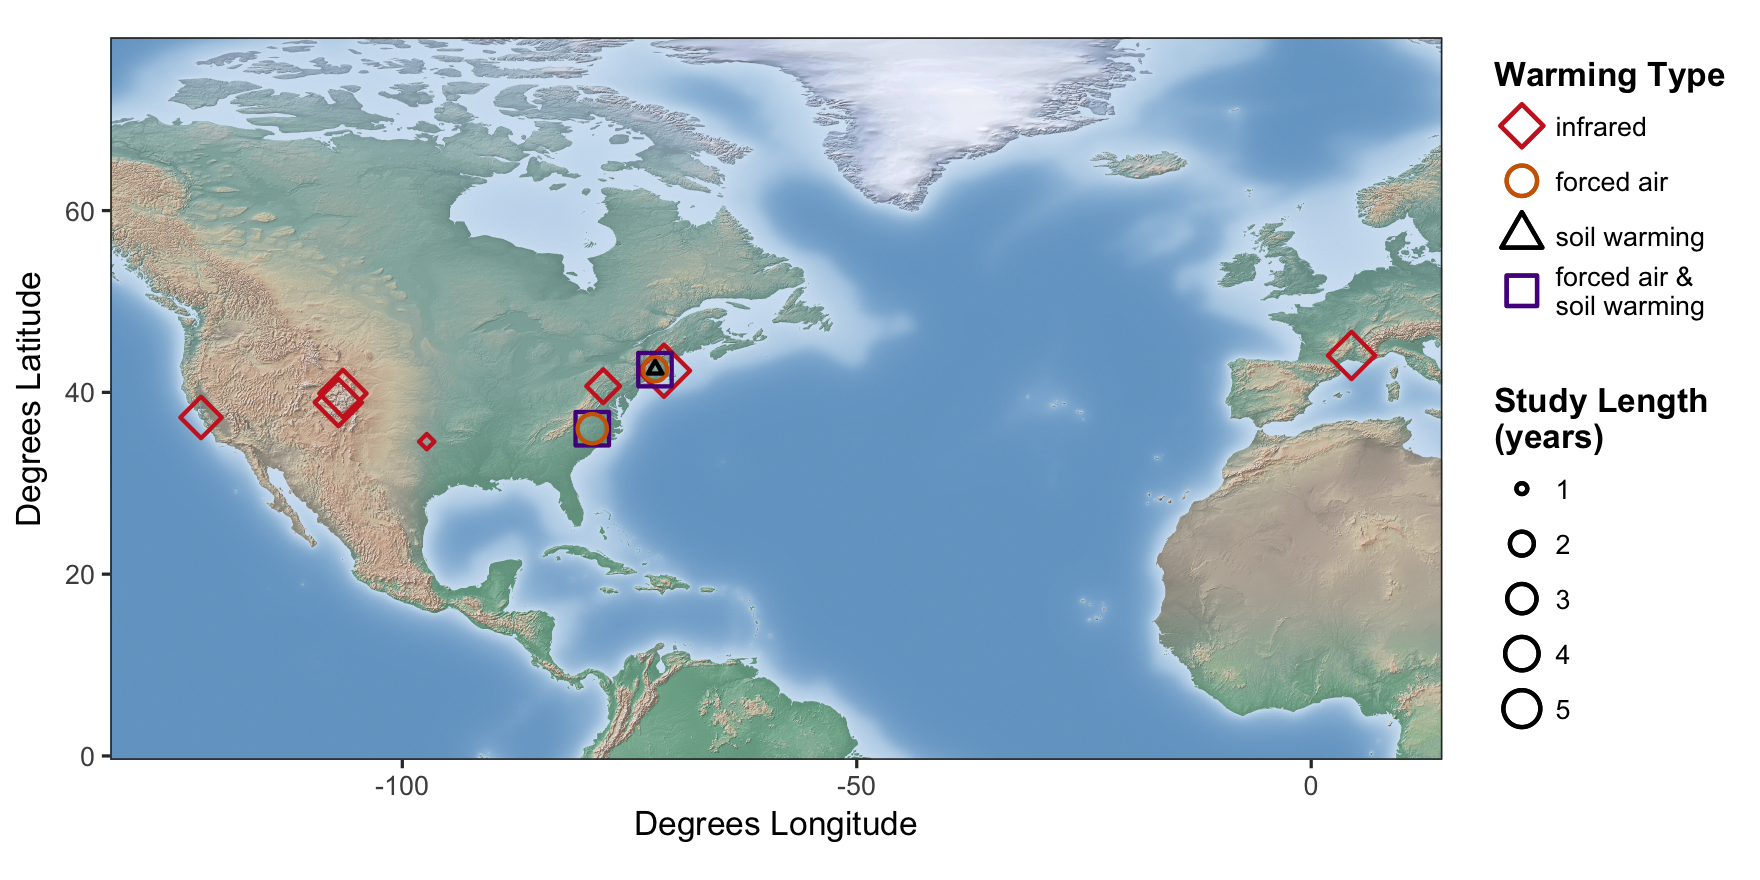
\includegraphics{/Users/aileneettinger/git/radcliffe/Analyses/maps/RadcliffeLocations_Experiments_Open.png} 
\caption{\textbf{Climate data from 15 climate change experiments in North America, Europe, and China are included in the MC3E database and analyzed here.} See Table \ref{tab:methods} for details.} 
\label{fig:map}
\end{figure}
\clearpage
\begin{figure}[h]
\centering
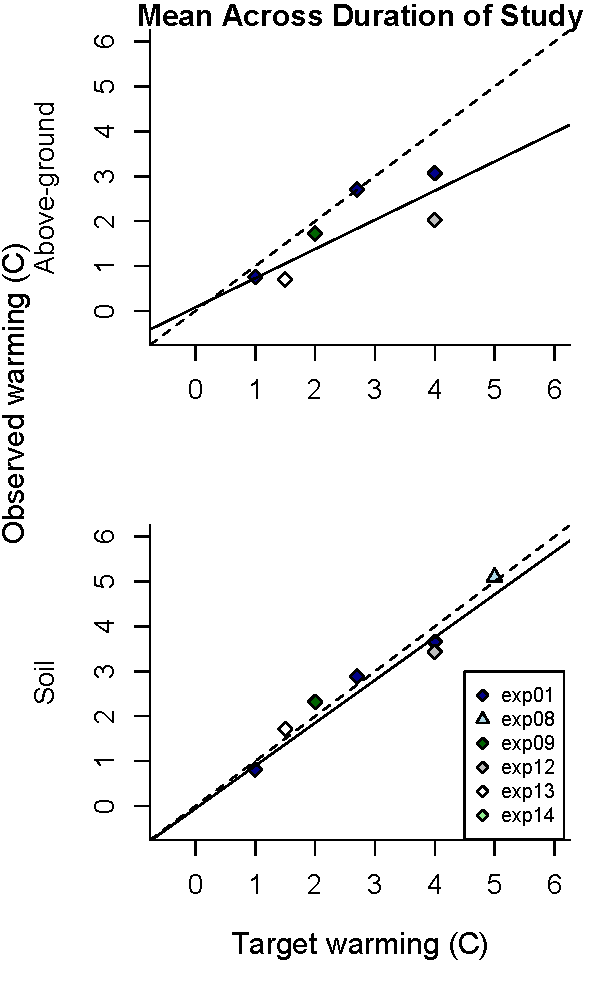
\includegraphics{/Users/aileneettinger/git/radcliffe/Analyses/figures/blockyearmean_target.pdf}
\caption{\textbf{Mean observed warming, for above-ground and soil temperatures,} excluding data from plots that manipulated precipitation. Above-ground temperature includes air, canopy, and surface temperature. Points represent the difference between treatment and control plots averaged across all plots within a treatment and study, over the duration of the study. The solid line is the fitted relationship between observed and target warming and the dashed line shows when observed warming is exactly equal to target warming (1:1). Colors vary by heating type: gray represents infrared; red represent soil warming cables. Compare to Figure 2 in the main text.}
 \label{fig:blockyear}
 \end{figure}
\clearpage
\begin{figure}[h]
\centering
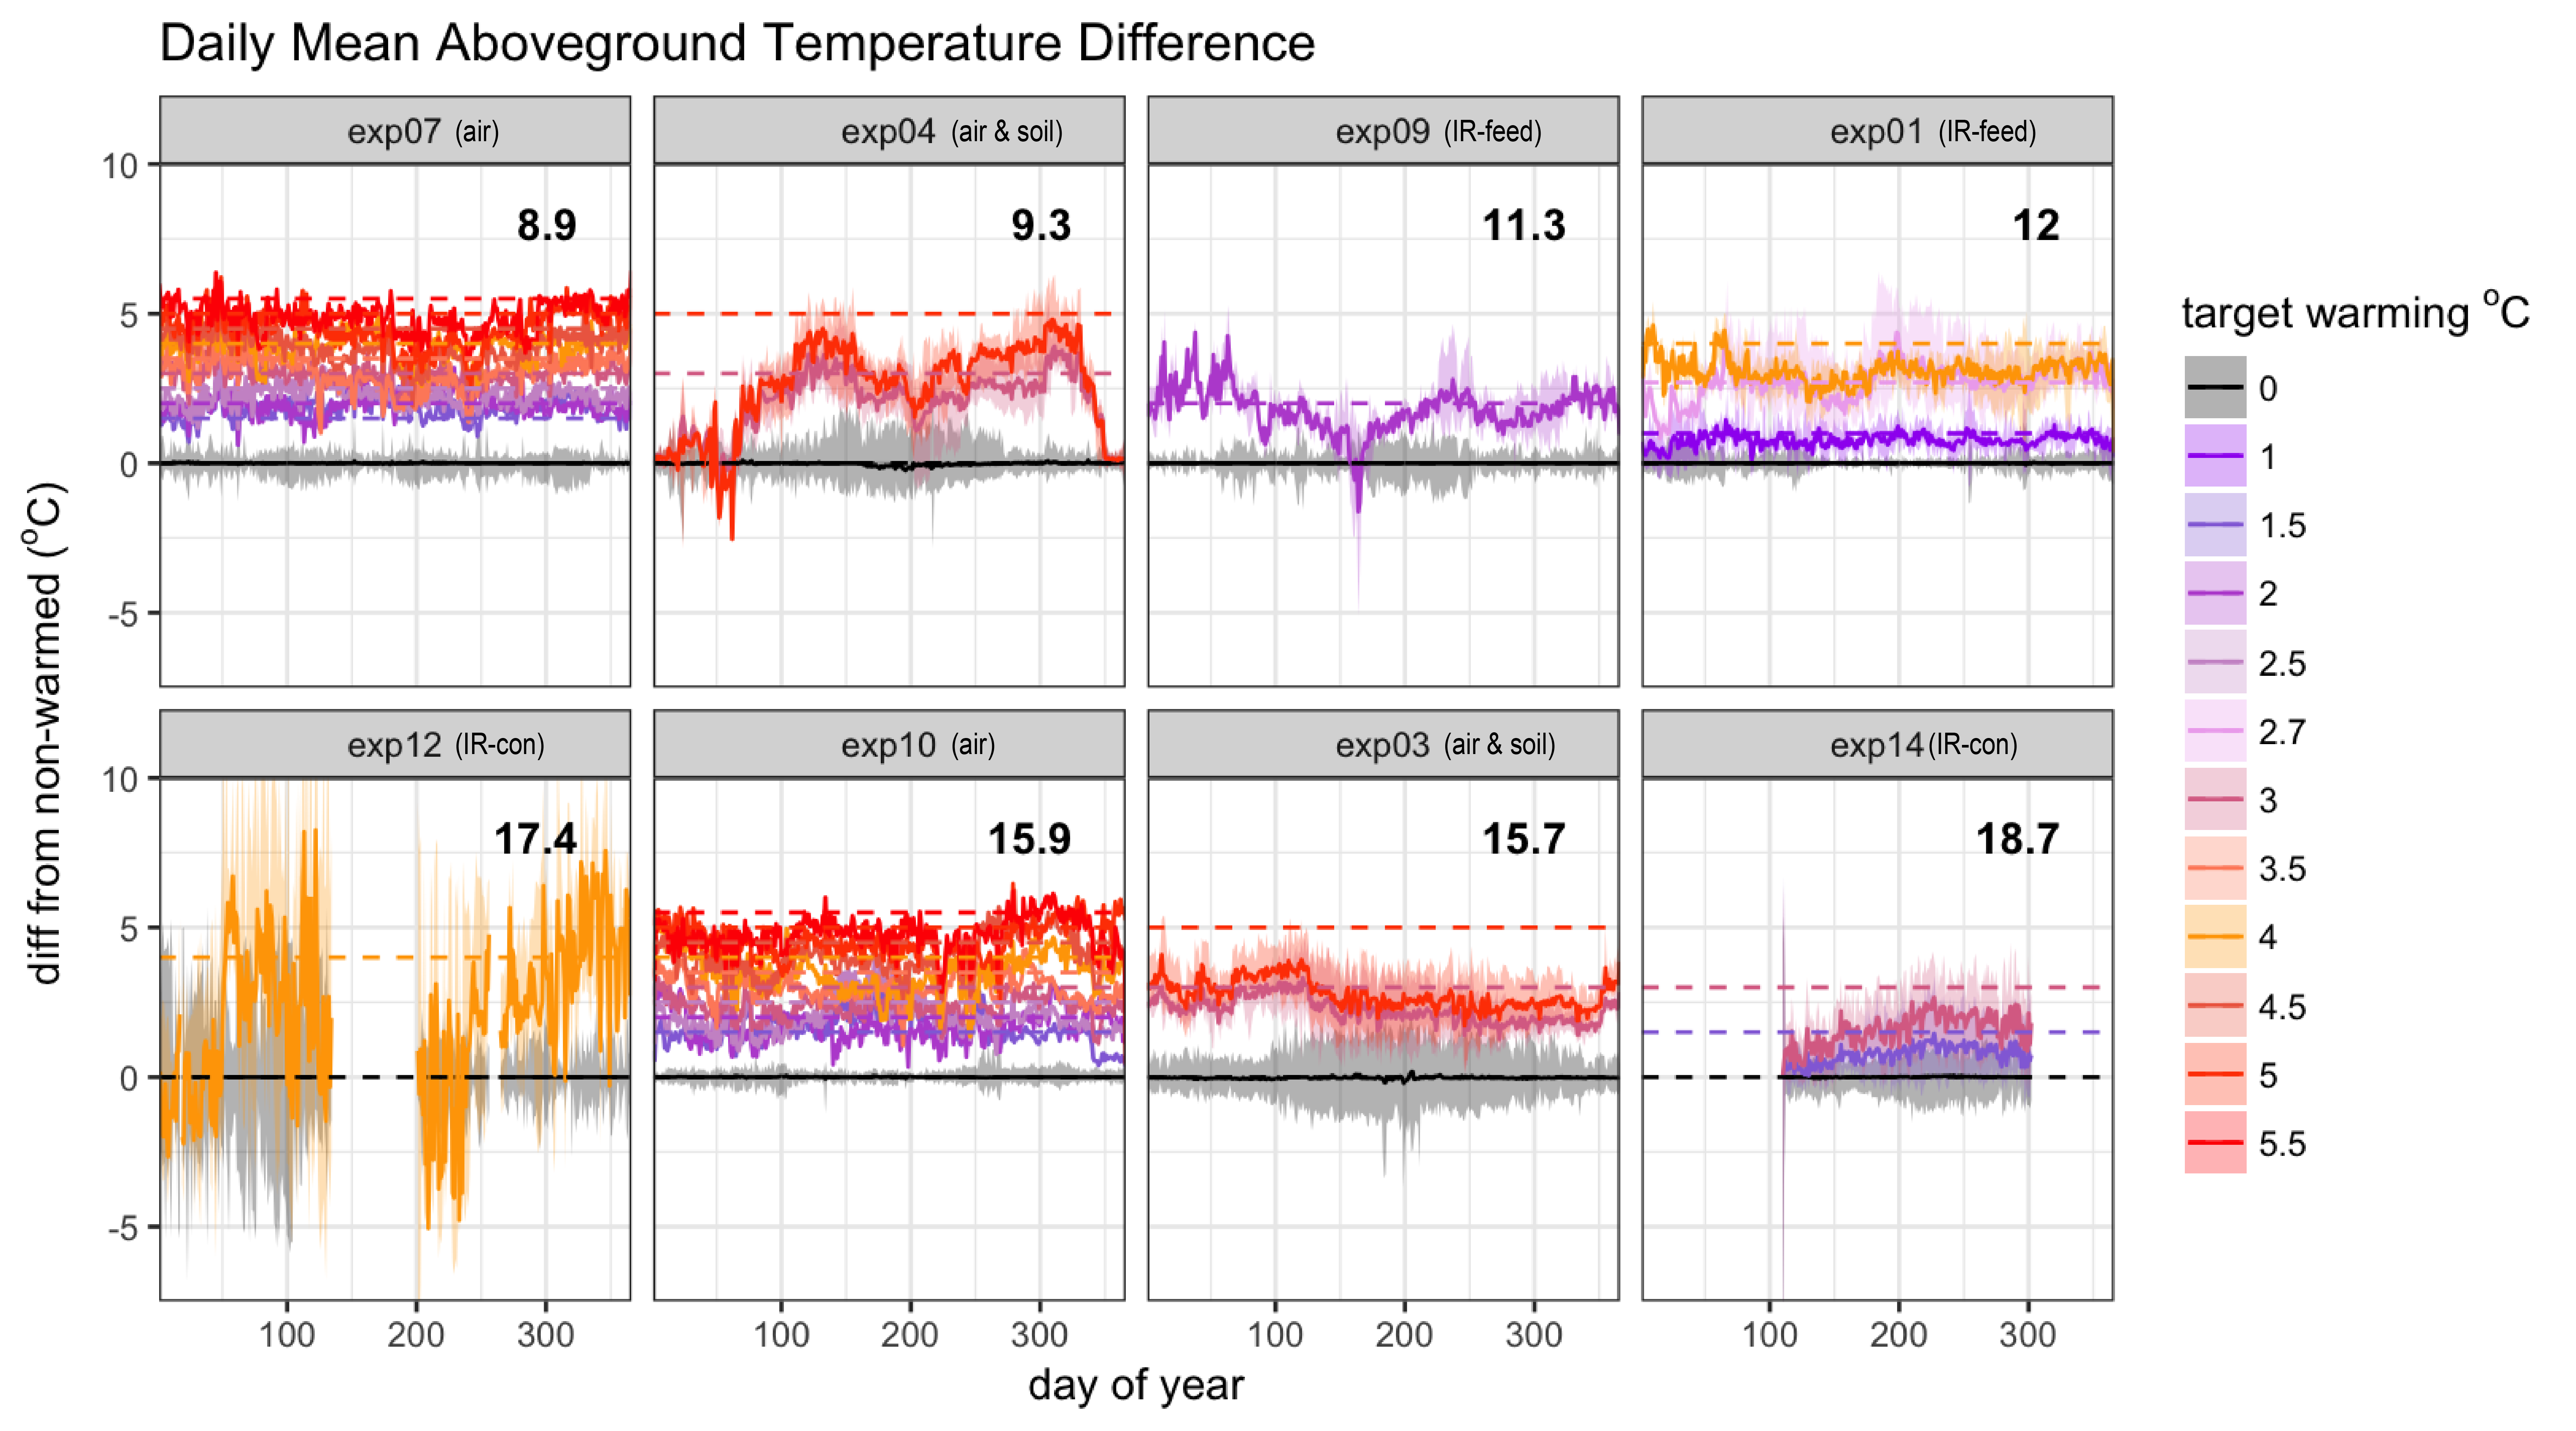
\includegraphics{/Users/aileneettinger/git/radcliffe/Analyses/figures/WarmingEffects_TimeSeries_AGTempMean_Deviation_NoPrecip_2.png}
\caption{\textbf{Deviations in daily observed warming from mean control above-ground temperature for 8 study sites,} excluding data from plots that manipulated precipitation. We show above-ground temperature, which includes studies that measured surface, canopy, and air temperature (see Table S1). Solid lines show observed difference between warming treatment (colors) and control (black) plots, averaged across replicates and years; shading shows 95\% confidence intervals. Dashed lines represent target warming levels. Experimental sites are ordered by low to high mean annual temperature (shown in the upper right corner of each panel). The heating type is listed in parentheses next to the site number (IR= infrared, soil= soil cables, air= forced air).} 
\label{fig:effwarmagtemp}
\end{figure}

% 
%%%%%%%%%%%%%%%%%%%%%%%%%%%%%%%%%%%%%%%
\end{document}
%%%%%%%%%%%%%%%%%%%%%%%%%%%%%%%%%%%%%%%%
